\documentclass{article}

\usepackage[numbers,sort&compress]{natbib}
\usepackage{graphicx}
\usepackage{doi}
\usepackage{hyperref}

\newcommand{\bemph}[1]{#1}

\usepackage{acronym}
\acrodef{agg}[AgFEM]{aggregated unfitted finite element method}
\acrodef{upc}[UPC]{Universitat Politècnica de Catalunya}
\acrodef{cimne}[CIMNE]{International Centre for Numerical Methods in Engineering}
\acrodef{lssc}[LSSC]{Large Scale Scientific Computing}
\acrodef{eccomas}[ECCOMAS]{European Community on Computational Methods in Applied Sciences}
\acrodef{semni}[SEMNI]{Sociedad Española de Métodos Numéricos en Ingeniería}
\acrodef{tum}[TUM]{Technical University of Munich}
\acrodef{lnm}[LNM]{Institute for Computational Mechanics}
\acrodef{amg}[AMG]{algebraic multigrid}
\acrodef{fsi}[FSI]{fluid-structure interaction}
\acrodef{dof}[DOF]{degree of freedom}
\acrodefplural{dof}[DOFs]{degrees of freedom}
\acrodef{fe}[FE]{finite element}
\acrodefplural{fe}[FEs]{finite elements}
\acrodef{pde}[PDE]{partial differential equation}
\acrodefplural{pde}[PDEs]{partial differential equations}
\acrodef{bddc}[BDDC]{balancing domain decomposition by constraints}


\begin{document}

\section{Post-doctoral research  at CIMNE (2016-present)} \label{sec:cimne}

\subsection{Introduction}

  This part of my research career starts in January 2016 and it extends up to the present. I joined \ac{cimne} as a post-doc researcher in 2016 and I was promoted to Assistant Research Professor in view of my academic results in 2019. In CIMNE, I am pursuing a research agenda, whose main objectives are:

\begin{itemize}
\item {\bf O1} Developing novel parallel \ac{fe} techniques for the simulation of complex problems in science an engineering using modern supercomputers
\item {\bf O2} Helping application experts to adopt these novel computational techniques to solve real-world problems
\item {\bf O3} Implementing these computer tools in open-souce software projects in order to foster their adoption by the scientific community
\end{itemize}


The main motivation underlying this research plan is the fact that many problems governed by \acp{pde} of interest in science and engineering are still nowadays computationally unaffordable. Complex predictive simulations require to resolve very different temporal and spatial scales, handle uncertainty in parameters and data, and couple different models, leading to expensive multi-physics computations. Fortunately, the rapid growth of available computer power based on multi-processor systems can open the door to drastically revert this situation, but brute computational force alone will not be enough. Nowadays, single-processor clock speeds have stagnated and any future computational power increase will be mainly achieved via parallelism. In consequence, most of the numerical methods developed in the last decades designed for single-processor systems will rapidly become obsolete. They will need to be replaced by next-generation highly scalable numerical algorithms. However, such techniques are still missing in many contexts and its development is expected to have a high impact in a wide range of disciplines. For this reason, I am tackling some of the current computational bottlenecks of \ac{fe} methods in large-scale parallel computations such as \ac{fe} mesh generation and the solution of discrete linear (and non-linear) problems resulting from the \ac{fe} discretization. This research in framed in three main research lines:


\begin{itemize}
\item {\bf RL1}  Simplify mesh generation in large-scale parallel computations via embedded \ac{fe} methods
\item {\bf RL2}  Software design of scientific applications and open-source projects
\end{itemize}

\subsection{RL1: Simplify mesh generation in large-scale parallel computations via embedded \ac{fe} methods}

\subsubsection{Research line description}


Mesh generation is known to be one of the main bottlenecks in real-world industrial \ac{fe} simulations. Conventional \ac{fe} methods require so-called body-fitted meshes, i.e., grids that conform to the geometrical boundaries of the computational domain (see Figure \ref{fig:fitted-vs-unfitted}). Constructing such grids is not obvious for complex geometries. It often requires skilled humans, and it is time consuming as mesh generation is estimated to be 80\% of total simulation time in industrial applications \cite{Cottrell2009}. The goal of so-called embedded \ac{fe} methods \cite{Badia2018,burman_cutfem:_2015,Schillinger2015} (also known as unfitted or immersed methods) is to change this situation by allowing one to work on background Cartesian meshes that do not necessarily conform to the geometrical boundaries (see Figure \ref{fig:fitted-vs-unfitted}). Generating such unfitted Cartesian grids is much simpler and more efficient that constructing body fitted meshes, specially in large parallel computations.  One can use highly scalable octree-based mesh generators like the p4est package \cite{burstedde_p4est_2011}, which has shown excellent scaling properties up to thousands of hundreds of CPU cores. 

\begin{figure}[ht!]
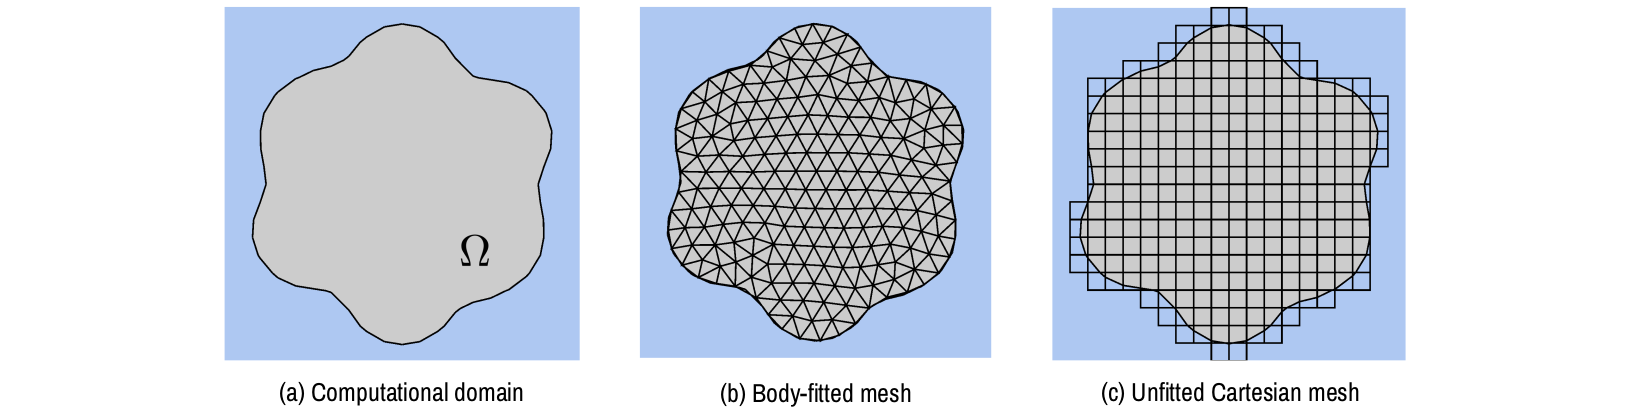
\includegraphics[width=\textwidth]{../_assets/fig1.png}
\caption{Body-fitted vs. unfitted meshes}
\label{fig:fitted-vs-unfitted}
\end{figure}


However, embedded methods have known drawbacks. One of the most notorious, still an open question today, is the so-called \emph{small cut cell problem}. Some cells of the unfitted mesh can be intersected by a very small part of the domain, which can lead to arbitrarily large condition numbers in the underlying discrete \ac{fe} operators \cite{DePrenter2017}. This is a major issue, when dealing with large-scale simulations that require Krylov sub-space iterative linear solvers \cite{saad_iterative_2003} because they are very sensitive to the conditioning and spectral properties of the underlying operators. The result is that embedded methods are mainly used in small to medium problems, which can be handled with direct linear solvers (i.e., Gaussian elimination) instead of iterative procedures. \bemph{One of my main research goals at \ac{cimne} is to address the conditioning problems of embedded methods in order to allow their usage in large-scale real-world computations}.


\subsubsection{Funding}

This research line has several funding sources. On the one hand, I was awarded with a Beatriu Pinós fellowship (a competitive post-doc grant issued by the Catalan autonomous government) to develop embedded \ac{fe} methods for the simulation of additive manufacturing processes. With the help of this grand I was able to develop new numerical techniques and mentor a PhD student in order to adopt these new tools in his additive manufacturing simulations. This work is also framed in the  H2020 project ``EMUSIC", which also focuses in the same application.  This research line  on embedded methods has also been supported by the  H2020 project ``ExaQUte". In particular, I am contributor in the work package ``WP1 Embedded methods", where I have lead the research associated with task ``Task 1.6: Development of robust (and scalable) linear solvers for the embedded case". Another funding source is the Spanish project  ``SOFAST".  I am involved in the works packages ``WP1 Embedded methods" and ``WP2 Adaptive mesh refinement". In the frame of these projects, I am currently supervising a PhD student at UPC, who is developing novel techniques to couple CAD models and embedded simulations.


\subsubsection{Results}

This research line has lead to several major research results, labeled Result-1.1-4, and detailed as follows.

\begin{itemize}
\item {\bf Result-1.1}  Multi-level domain decomposition for embedded \acp{fe}
\item {\bf Result-1.2} The aggregated unfitted \ac{fe} method (AgFEM)
\item {\bf Result-1.3} Extension of AgFEM to large-scale parallel and adaptive computations
\item {\bf Result-1.4} Embedded \ac{fe} methods for 3D printing simulations
\end{itemize}

\paragraph{Result-1.1: Multi-level domain decomposition for embedded \acp{fe}.} \label{sec:unf-BDDC}


In \ac{fe} analysis, the current way to solve linear systems at large-scales is using iterative Krylov sub-space methods in combination with parallel and scalable preconditioners. Unfortunately, existing preconditioners like \ac{amg} \cite{Briggs2000} or multi-level domain decomposition \cite{Toselli2005} are mainly designed for body-fitted meshes and cannot readily deal with the ill-conditioning associated with small cut cells. 

Specific precontinoners for unfitted methods have been proposed in the literature in different contexts (see, e.g., \cite{berger-vergiat_inexact_2012,DePrenter2017,hiriyur_quasi-algebraic_2012,menk_robust_2011} ). However, they are mainly serial non-scalable algorithms.  This has motivated me to develop novel techniques in order to enable the usage of embedded method in much larger computations. As a first approach, I have considered \ac{bddc} preconditioners to solve such problems at large scales. This choice is motivated by the fact that \ac{bddc} methods are among the most scalable preconditioners for \ac{fe} analysis. In particular, the \ac{bddc} methods implemented in FEMPAR \cite{badia_fempar:_2017} have shown an excellent weak scaling up to 458,752 cores and 30 billion unknowns \cite{badia_multilevel_2016}. Unfortunately, conventional \ac{bddc} preconditioners loose they optimal qualities, when the underlying problem is discretized with an unfitted grid. Thus, available \ac{bddc} solvers cannot be considered in combination with embedded \ac{fe} methods. 

In order to revert this unfavorable situation, {{I have introduced a novel \ac{bddc} method  specifically tailored to deal with embedded grids}}. The proposed method is based on a modification of the coarse space of the \ac{bddc} solver,  which makes it robust with respect to badly cut cells. The method has been shown to be algorithmically weak scalable for a wide range of 3D complex geometries. That is, the number of iterations needed to reach convergence in the preconditioned linear solver is asymptotically independent of the problem size (see Figure \ref{fig:fitted-vs-unfitted-bddc}). This work has motivated the {{publication of 1 paper in a Q1 ranked journal}} (see reference \cite{badia_robust_2017}), and has been presented in several conferences both at national and international level.

\begin{figure}[ht!]
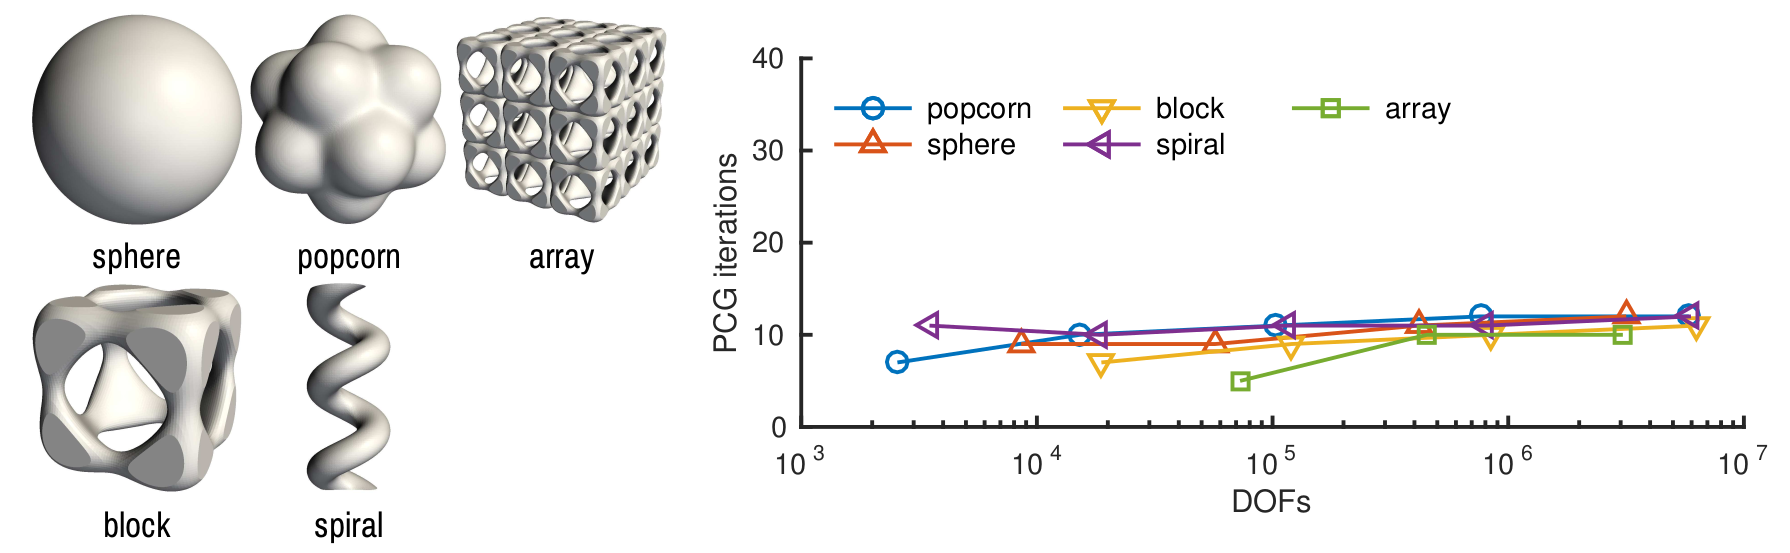
\includegraphics[width=\textwidth]{../_assets/fig2.png}
\caption{BDDC for embedded methods in a weak scaling test for a Poisson problem on different complex  3D geometries. A perfect weak scaling of the linear solver iterations is obtained.}
\label{fig:fitted-vs-unfitted-bddc}
\end{figure}

\paragraph{Result-1.2: The aggregated unfitted \ac{fe} method (AgFEM).}

Most of the works enabling the usage of iterative linear solver in combination with embedded \ac{fe} methods consider tailored preconditioners in order to deal with matrices affected by the small cut cell problem (e.g., the \ac{bddc} method for embedded grids previously presented in Section \ref{sec:unf-BDDC}). The main drawback of this approach is that one relies on highly customized solvers, and therefore, it is not possible to take advantage of well known and established linear solvers for \ac{fe} analysis available in renowned scientific computing packages as Trilinos \cite{Heroux2005} or PETSc \cite{petsc-user-ref}. In order to address this issue, I have considered a second approach. \bemph{I have developed an enhanced \ac{fe} formulation that leads to linear systems, whose condition number is not affected by small cuts} (see Figure \ref{fig:aggfem}). Therefore, they can be solved with standard linear solvers such as the \ac{amg} \cite{Baker2011} methods available in Trilinos or PETSc.

The enhanced \ac{fe} formulation is called \ac{agg}, which is based on removal of shape functions associated with badly cut cells by introducing carefully designed constraints.  The formulation of \ac{agg} shares the good properties of body-fitted \ac{fe} methods such as stability, condition number bounds, optimal convergence, and continuity with respect to data.  In contrast to previous works like CutFEM \cite{burman_cutfem:_2015}, it is easy to implement and to use in different problem types since it does not require to compute high order derivatives of the shape functions, and it does not introduce extra dissipation terms in the weak form.  \ac{agg} has already been successfully applied to the solution of fluid \cite{Badia2018a} and heat transfer problems \cite{Badia2018}. This work has lead to {{2 publications in Q1 journals}} (references \cite{Badia2018,Badia2018a} ) and several conference contributions at national and international level. Find in Figure \ref{fig:complex-case1-sol} a flow simulation using the \ac{agg} method.

\begin{figure}[ht!]
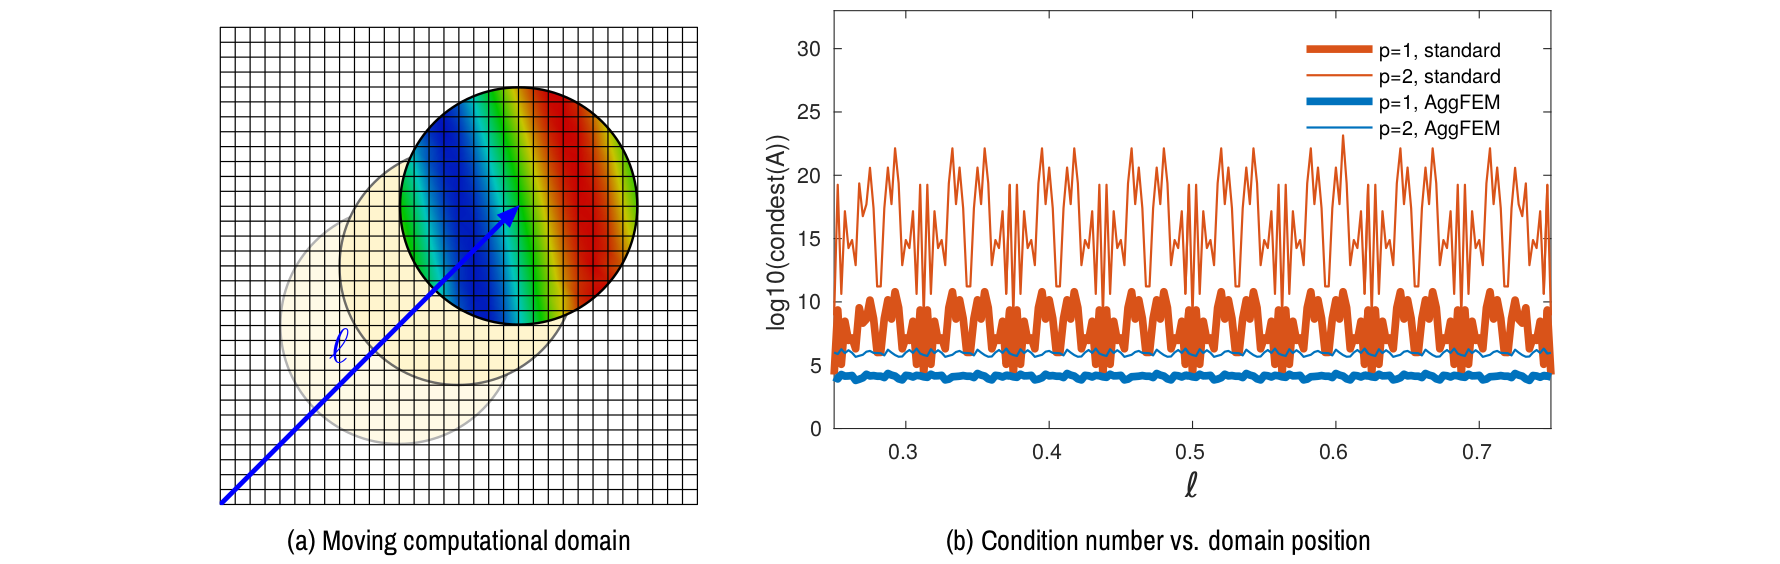
\includegraphics[width=\textwidth]{../_assets/fig3.png}
\caption{Poisson problem defined on a moving domain. Note that the standard embedded formulation leads to very high condition numbers, which are very sensitive to the relative position between the computational domain and the background mesh, specially for second order interpolations ($p=2$). In contrast, the condition number is much lower for the enhanced formulation (the \ac{agg} method) and it is nearly independent of the position of the domain.}
\label{fig:aggfem}
\end{figure}


\begin{figure}[ht!]
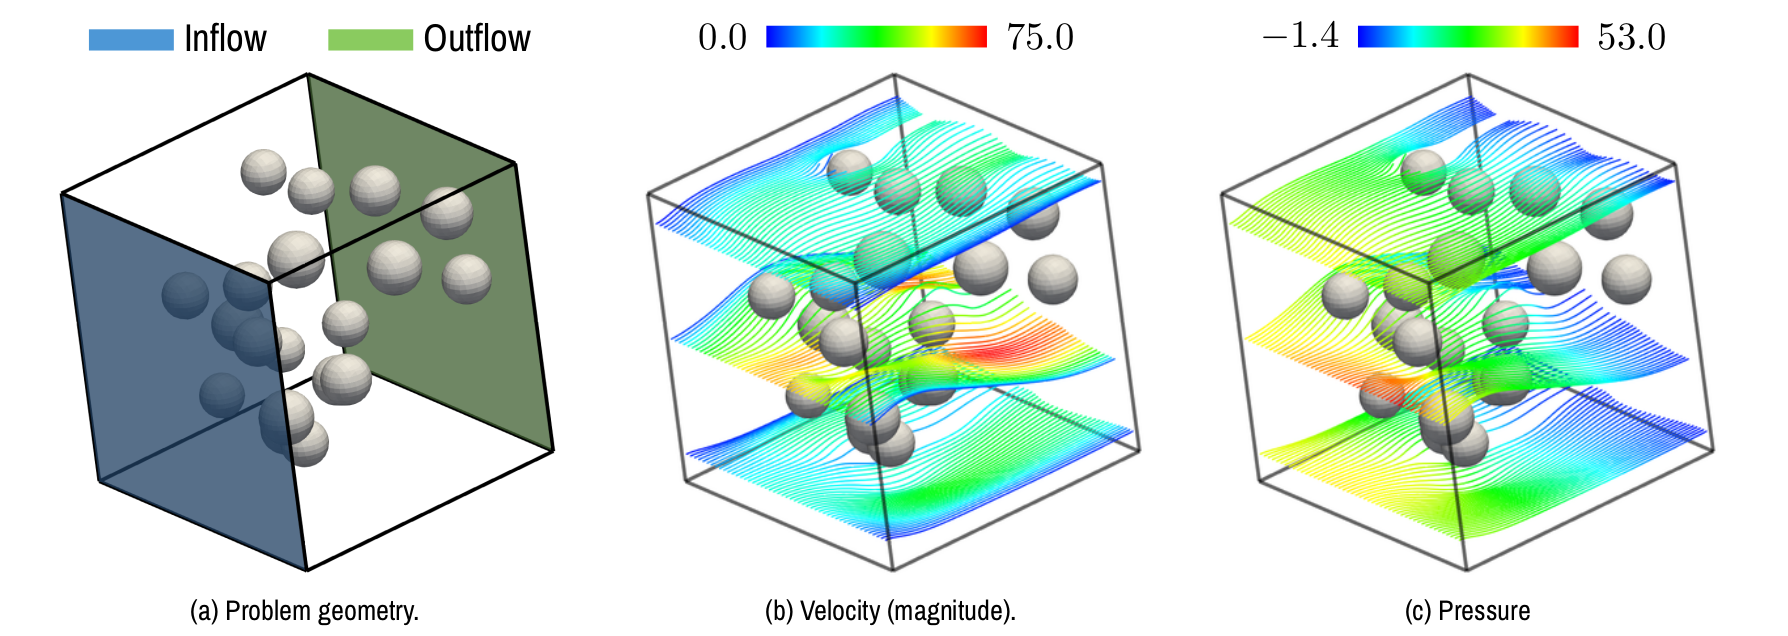
\includegraphics[width=\textwidth]{../_assets/fig4.png}
  \caption{Numerical solution of a (dimensionless) Stokes problem using the \ac{agg} method (streamlines colored by velocity magnitude and pressure). This computation is carried out without constructing an unstructured body-fitted mesh thanks to the application of the \ac{agg} method.}
  \label{fig:complex-case1-sol}
\end{figure}



\paragraph{Result-1.3: Extension of AgFEM to large-scale parallel and adaptive computations.}

I have implemented a distributed-memory version of \ac{agg} in the FEMPAR software project by making use of MPI for inter-processor communications. The obtained results confirm my expectations. When using \ac{agg}, the resulting systems of linear algebraic equations can be effectively solved using standard \ac{amg} preconditioners. In this case, I have considered the \ac{amg} methods available in the GAMG module of the PETSc library. {{With the parallel \ac{agg}, I was able to run  weak scaling tests up to  300M \acp{dof} and 16K processors in the Marenostrum-IV platform}}. The results show that the optimal behavior of \ac{amg} solvers for body-fitted meshes is also recovered for \ac{agg}, i.e. number of linear solver iterations asymptotically independent of problem size. To my best knowledge, this is the first time that embedded methods are successfully applied to such large scales. These results have been published in a { Q1 international jounral} (see reference \cite{Verdugo2019}).

Parallel implementations and scalable solvers are essential to dramatically reduce the computation times of challenging simulations, but not sufficient in many contexts. Several problems of interest are multi-scale in nature and, thus, require different mesh resolution in different spatial locations. In this context, trying to capture the finest scales with uniform meshes in overkill and the usage of adaptive mesh refinement becomes mandatory.

 Parallel mesh adaptation is a challenging operation since mesh partition and load balance needs to be carefully realized to achieve performance.  In large parallel computations, Cartesian grids locally adapted with forest-of-trees (also known as octree meshes) are among the few ways to locally adapt in a scalable way. They leverage so-called \emph{space-filing curves} \cite{Holke2018} to reduce the mesh partition and load balance to a 1d problem that can be solved very efficiently. However, the main drawback of this approach is that the resulting computational grid contains so-called \emph{hanging nodes}, which require extra work when defining conforming \ac{fe} interpolations. If certain conditions are not satisfied, the constraints introduced by hanging nodes may expand beyond a single layer of ghost cells, thus leading to an incorrect parallel FE solver. Unfortunately, the current literature fails to explain under which conditions this happens for generic conforming \ac{fe} discretizations (i.e., not only limited to Lagrangian elements). To address this situation, I have studied the correctness of a number of algorithms and parallel data structures needed to build conforming \ac{fe} discretizations on octree meshes partitioned via space-filling curves.  The proposed algorithms and data structures have been implemented within the FEMPAR scientific software library~\cite{badia_fempar:_2017}, using p4est \cite{Bangerth2007} as the forest-of-trees back-end. A strong scaling study reveals remarkable scalability up to 32.2K CPU cores and 482.2M \acp{dof}. {This work has been recently published in the Q1 journal ``SIAM Journal on Scientific Computing"} (see reference \cite{Badia2019a} ).

 In a second step, I have combined the parallel AgFEM implementation previously developed with this adaptive \ac{fe} framework. The result is a novel scalable distributed-memory version of AgFEM on locally-adapted Cartesian meshes. The main novelty of the method is a two-step algorithm that carefully mixes AgFEM constraints, which get rid of the small cut cell problem, and standard hanging node constraints, which ensure trace continuity. This method requires minimum parallelization effort since it can leverage standard functionality available in existing large-scale \ac{fe} codes. Numerical experiments demonstrate its optimal mesh adaptation capability, robustness to cut location and parallel efficiency, on classical Poisson hp-adaptivity benchmarks. This work opens the path to functional and geometrical error-driven dynamic mesh adaptation with the \ac{agg} method in large-scale realistic scenarios. A research paper detailing this work is published in reference \cite{Badia2020a}).

\paragraph{Result-1.4: Embedded \ac{fe} methods for 3D printing simulations.}

One the main driving applications of my research on embedded \ac{fe} methods is {{the simulation of additive manufacturing processes using advanced large-scale \acp{fe}}}. This is the main topic of my Beatriu Pinós fellowship and the {{EU H2020 project "EMUSIC"}}, were I have participated as researcher. Additive manufacturing (also known as 3D printing) is an advanced manufacturing method used to build physical objects directly from 3D computer designs by the superposition of thin layers of materials such as metals, polymers or composites. 3D printers have been described in numerous occasions as a revolutionary technology with the potential to radically transform the manufacturing industry. However, high-energy sources used to melt metal powders during the printing process induce thermo-mechanical shape distortions and residual stresses, that deteriorate the geometrical quality and the requested material properties. Currently, the standard industrial practice  to optimize the printing process in order to obtain quality components is through experimental testing, which is expensive and time consuming since it requires the production of hundreds of prototypes before reaching the final piece. Fortunately, predictive computer simulations can potentially be used to validate the process parameters before printing the component. However, current simulation software still has important limitations when it comes to predict shape distortions and residual stresses in complex settings with an acceptable level of accuracy and an acceptable time frame. 

\begin{figure}[ht!]
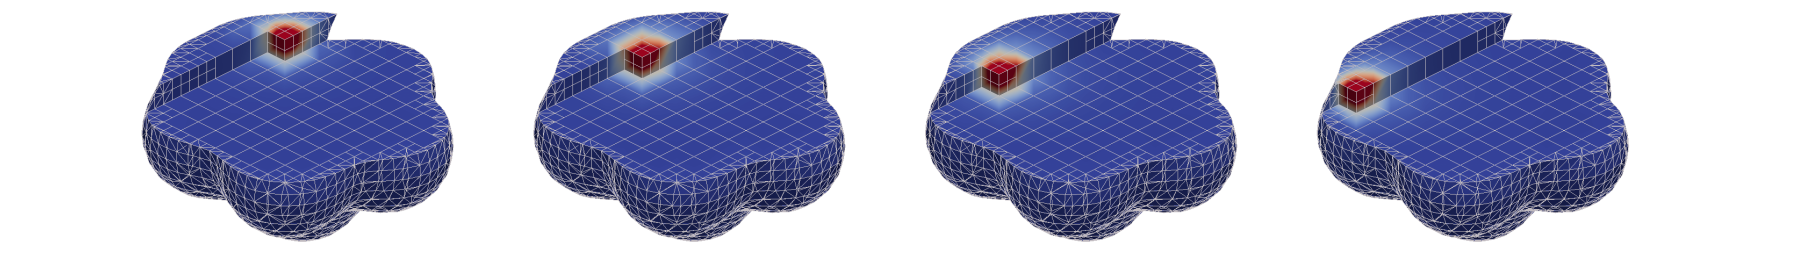
\includegraphics[width=\textwidth]{../_assets/fig6.png}
\caption{Snapshots of a thermal 3D printing simulation using the \ac{agg} method in order to effectively represent the geometry of the growing piece.}
\label{fig:AM-AggFEM}
\end{figure}

I have contributed to develop novel computational tools able to provide much faster and accurate results. In particular, generating computational meshes for additive manufacturing simulations is particularly challenging and time consuming. The shape of the 3D printed object grows in time, layer-by-layer, as it is produced. Capturing the growing shape requires a different mesh for each time step to represent the portion of the piece that has been produced so far. It is obvious that generating thousands of independent meshes with conventional methods is virtually impossible.  Thus, embedded methods are well suited in this context. {{I have applied the \ac{agg} method to additive manufacturing simulations}} in collaboration with a PhD student of my research team (see Figure \ref{fig:AM-AggFEM}). %They have been recently presented in the "Additive Manufacturing Benchmarks 2018" conference in the USA. This work will motivate a journal publication in the near future.

\subsubsection{Current and future work}

 I plan to continue working on my current research line on large-scale \ac{fe} solvers and embedded  methods and its application to challenging engineering problems. I will extend these techniques to more challenging problem types and collaborate with application experts in order to simulate relevant real-world cases.
 
 

\subsection{RL2: Software design of scientific applications and open-source projects}

\subsubsection{Research line description}

I have recently started a new research line whose goal is to develop a new generation of open-source \ac{fe} codes that leverages the latest advances in compilers and programming languages.  The development of high-performance scientific software for the numerical approximation of \acp{pde} is a key research area with a broad impact in advanced scientific and engineering applications. Existing \ac{pde} solvers like \ac{fe} codes are usually written in compiled programming languages introduced several decades ago, mainly C/C++ and Fortran 95/03/08. These languages are considered for performance reasons, but they are also related to poor code productivity. In contrast, interpreted languages like Python or MATLAB allow one to write scripts and applications in much less lines of code, boosting code productivity, but they lead to much slower programs. A trade-off between performance and productivity is usually achieved in scientific software libraries like deal.ii \cite{Bangerth2007} or FEniCS \cite{Alnaes2015} by combining an efficient C/C++ computational back-end with a user-friendly high-level Python user front-end. However, this approach is not satisfactory, when researchers need to extend these libraries with new features since they are forced to learn and modify a complex C/C++ back-end instead of benefiting from the productivity expected from the Python front-end. This problem is referred to as the \emph{two-language problem}.

Fortunately, recent advances in compiler technology are starting to revert this situation. In the field of scientific computing, Julia \cite{Bezanson2017} is a new computer language that combines the performance of compiled languages with the productivity of interpreted ones by using recent advances in compiler technology like type inference and just-in-time compilation. As a result, the same language can be used both for the back-end and the front-end, thus eliminating the two-language problem. Based on this novel paradigm, I have started the Gridap.jl project \cite{Badia2020}, a new generation, open-source, \ac{fe} framework completely written in the Julia programming language. Gridap.jl allows users to write \ac{fe} applications in a notation almost one-to-one to the mathematical notation used to define the \ac{pde} weak form. For instance, see, in Figure \ref{fig:gridap-code}, how a Poisson equation on a complex 3D domain can be solved in Gridap.jl with few lines of code. To my best knowledge, only libraries like FEniCS are able to achieve such compact user interfaces, but they are based on sophisticated compilers of variational forms \cite{Kirby2006}, which generate, compile and link a specialized C++ back-end for the problem at hand. One of the limitations of this approach is that form compilers are rigid systems, not designed to be extended by average users. In contrast, Gridap.jl is based on a much simpler approach. It leverages the Julia just-in-time compiler to generate efficient problem-specific code without the need to maintain a custom compiler of variational forms.

\begin{figure}[ht!]
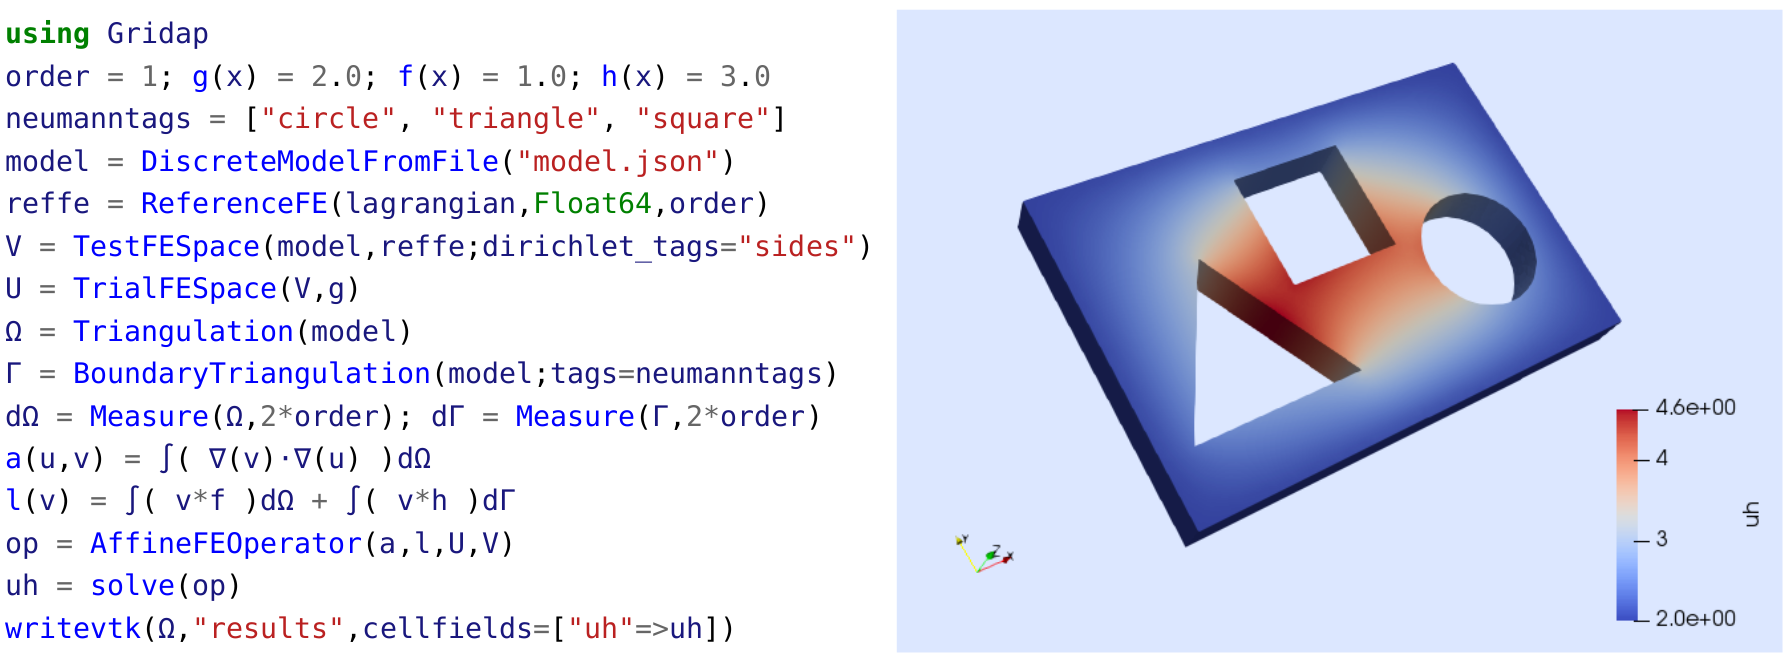
\includegraphics[width=\textwidth]{../_assets/fig11.png}
\caption{User code to solve a 3D Poisson equation in Gridap.jl and view of the corresponding numerical solution. Note that the bilinear and linear forms of the problem, \texttt{a} and \texttt{l}, are specified with a syntax closely related to their mathematical notation thanks to an advanced software design based on the Julia computer language. The file containing the discrete model can be downloaded from \url{https://github.com/gridap/Tutorials/raw/master/models/model.json} in order to execute this code snipped.} 
\label{fig:gridap-code}
\end{figure}

\subsubsection*{Funding}

Gridap.jl appears as one of the two  \ac{fe} codes selected to implement new novel \ac{fe} methods in a { "Discovery Project" of the Australian Research Council} (ref: DP210103092, \$475000) co-lead by my collaborator at Monash University Prof. Santiago Badia. In the framework of this project, new collaborators are expected to joint and contribute in the expansion of the project. In addition, Gridap.jl has been accepted as a {NumFOCUS affiliated project} (\url{https://numfocus.org/}). The mission of NumFOCUS is to promote open practices in research, data, and scientific computing by serving as a fiscal sponsor for open source projects and organizing community-driven educational programs. Being an affiliated project, Gridap.jl is eligible to participate in NumFOCUS funding schemes and other events like the participation in the Google Summer of Code (\url{https://g.co/gsoc/}) under the NumFOCUS umbrella.

\subsubsection*{Results}

\begin{itemize}
\item {\bf Result-2.1} Initial release of the open-source \ac{fe} project Gridap.jl
\item {\bf Result-2.2} GridapEmbedded.jl: a Gridap.jl plugging providing embedded \ac{fe} methods
\end{itemize}

\paragraph*{Result-2.1: Initial release of the open-source \ac{fe} project Gridap.jl.} 

The first immediate result in this research line is the initial release of the project, whose source code is freely available at github (\url{https://github.com/gridap/Gridap.jl}) under a MIT software license. In addition, a related article  {has been published in the ``Journal of Open Scientific Software"} (see reference \cite{Badia2020}). Gridap.jl is already a fully functional general-purpose \ac{fe} library ready to solve linear, non-linear, steady-state, and time-dependent \acp{pde}. It already provides different types of conforming \ac{fe} methods like nodal Lagrangian elements for grad-conforming approximations (e.g., for linear elasticity or thermal analysis) or non-nodal interpolations like Raviart-Thomas for div-conforming approximations (e.g., for flow in porous media). Discontinuous Galerkin schemes are also supported. Gridap.jl is currently used by several research groups worldwide in institutions such as Monash University, MIT, TU Delft, UPC, and CIMNE. A set of introductory tutorials to the library is available at \url{https://github.com/gridap/Tutorials} and a live chat to ask questions and interact with the Gridap.jl community is available at \url{https://gitter.im/Gridap-jl/community}.

\paragraph*{Result-2.2: GridapEmbedded.jl: a Gridap.jl plugging providing embedded \ac{fe} methods.}

The Gridap.jl project is designed to be an extensible package ecosystem with several plugins that extend the functionality of the core repository. In particular, GridapEmbedded.jl (\url{https://github.com/gridap/GridapEmbedded.jl}) is an extension that implements embedded \ac{fe} methods. At this moment, it provides embedded methods based on classical ghost-penalty \cite{burman_cutfem:_2015} or methods based on \ac{agg}. GridapEmmbedded.jl will be the basis to implement the new space-time methods proposed in Task-1.2 since it is implemented in a dimension-implemented fashion allowing to consider 4D meshes in the future. 

\subsubsection*{Future work}
 
 
\paragraph*{GridapDistributed.jl: a  Gridap.jl plugging for parallel distributed computations.} 

At this moment, Gridap.jl provides mainly serial algorithms and needs to be extended to parallel computations in order to cope with large-scale realistic simulations. To this end, I have started the plugin GridapDistributed.jl (\url{https://github.com/gridap/GridapDistributed.jl}), whose goal is to provide the parallel functionality needed in parallel distributed-memory computations. I am designing a set of extensible distributed data structures that allow one to implement parallel algorithms in a generic way independent on the parallel computing environment (e.g., MPI or the Julia build-in distributed mode) used to run the computations. This is specially handy for developing new code since it allows one to debug parallel algorithms by running an emulated distributed computation in a standard (sequential) Julia session and using standard serial debuggers.  Once the code works with the emulated parallel mode, it can be automatically deployed in a supercomputer via an MPI back-end implemented for this purpose. Thus, the package provides a very convenient way of developing parallel algorithms, while achieving the performance of MPI-based applications. This will help to develop new parallel \ac{fe} methods (like the parallel extension of the space-time AgFEM methods described in Task-1.2) in a very effective way. In particular, PhD students not necessarily experts in the MPI library can benefit from this framework to develop their parallel algorithms. At this moment, I have been able to solve the Poisson equation with up to 1B cells on 16K processors with GridapDistributed.jl on Gadi (an Australian super-computer) and I expect to further mature and extend the capabilities of this library.  
 
\paragraph*{Leveraging the Gridap.jl ecosystem to solve problems in science and engineering.}

Several researchers have already realized the potential benefits of using the Gridap.jl framework for their applications and have asked to me for collaboration. My plan is to grow a network of scientific collaborators that use the library in several contexts, in order to increase my changes of publishing more research papers and to find relevant topics for preparing project proposals.





\section{Post-doctoral research at TUM (2013-2015)} \label{sec:tum}

In this post-doc stay, \bemph{I have developed parallel \ac{amg} solvers for the solution of large systems of linear algebraic equations associated with the \ac{fe} discretization of complex multi-physics problems}.  The main goal of this research was to provide a general framework able to be applied to several problem types. In particular, this work was applied to \ac{fsi}, thermo-mechanical coupling, and human respiratory mechanics among others.

\subsection{General framework for the solution of coupled problems with monolithic schemes}

The numerical simulation of coupled problems via discretization techniques such as the \ac{fe} method requires special solution strategies for solving the coupling between
the underlying physical fields. The so-called partitioned methods \cite{Felippa2001} are often the preferred choice in industrial applications because they allow to reuse existing (black-box) solvers for the individual fields. However, this approach is unstable for many challenging strongly coupled problems \cite{Causin2005,Forster2007} and, therefore, another family of methods called monolithic are required in a variety of complex settings. It has also been shown that monolithic schemes are often preferable in terms of efficiency as compared to partitioned ones. For that reason, this approach has been the preferred option for solving many strongly coupled problems in the literature, see e.g. \cite{Badia2008,badia_block_2014}. However, the price to be paid for the extra robustness of monolithic methods is a more challenging system of linear equations. The system matrix is a big sparse matrix with a special block structure representing each of the underlying physical fields and frequently has a very bad condition number. In real-world applications, iterative methods such as GMRES \cite{saad_iterative_2003} are used to attack this linear system, which requires efficient preconditioners for addressing the bad conditioning of the problem. Selecting a suitable preconditioner is the key point in the solution process.

The conventional approach to design preconditioners for coupled problems is to use approximated block inverses in order to untangle the coupling between the physical fields, and then, to use efficient \ac{amg} solvers for the resulting uncoupled problems. The drawback of these methods is that the coupling is resolved only at the finest grid level. Thus, using efficient \ac{amg} solvers for the underlying problems does not necessarily imply a good treatment of the coupling and a fast global solution. This drawback is overcome by Gee et al. \cite{Gee2011}, who propose an enhanced block preconditioner (referred to as monolithic \ac{amg}) for \ac{fsi} applications, which enforces the coupling at all grid levels, and often results in a better solver performance. Monolithic \ac{amg} preconditioners are a promising approach for other coupled problems as well but, this strategy was only applied to \ac{fsi}. In order to allow the usage of this enhanced \ac{amg} methods for a wide range of problem types, \bemph{I have developed an general computational framework based on monolithic \ac{amg} techniques}. For comparison purposes, conventional \ac{amg} solvers were also included. The method was implemented in the high performance multi-physics code BACI \cite{Wall2014} and \bemph{it was published in a Q1 journal} (see reference \cite{verdugo_unified_2016}). This framework has been used at \ac{tum} since then, and \bemph{it has been considered by several papers in top international journals} (see, e.g., \cite{Kremheller2018,Fang2018}), with a wide range of applications including  simulation of vascular tumor growth and simulations of lithium ion cells.


%A monolithic, mortar‐based interface coupling and solution scheme for \ac{fe} simulations of lithium‐ion cells
%
%A monolithic multiphase porous medium framework for (A-) vascular tumor growth
%
%A Nitsche-based cut \ac{fe} method for the coupling of
%incompressible fluid flow with poroelasticity
%
%Monolithic cut \ac{fe} based approaches for fluid-structure interaction
%
%A consistent approach for fluid-structure-contact interaction based on a porous flow model for rough surface contact


\subsection{Solvers for the thermo-mechanical coupling in rocket nozzles}

In the framework of the \bemph{German research project} ``Fundamental Technologies for the Development of Future Space-Transport-System Components under High Thermal and Mechanical Loads", I have applied the general linear solver framework to the simulation of the thermo-mechanical coupling in rocket nozzles. I exemplary show here the performance of the developed preconditioners. The nozzle geometry  (see Figure \ref{fig:tsi-rocket-geom}) and other problem parameters are inspired by the ``Vulcain" rocket engine installed in the Ariane space launcher, see  \cite{verdugo_unified_2016} for further details.

\begin{figure}[ht!]
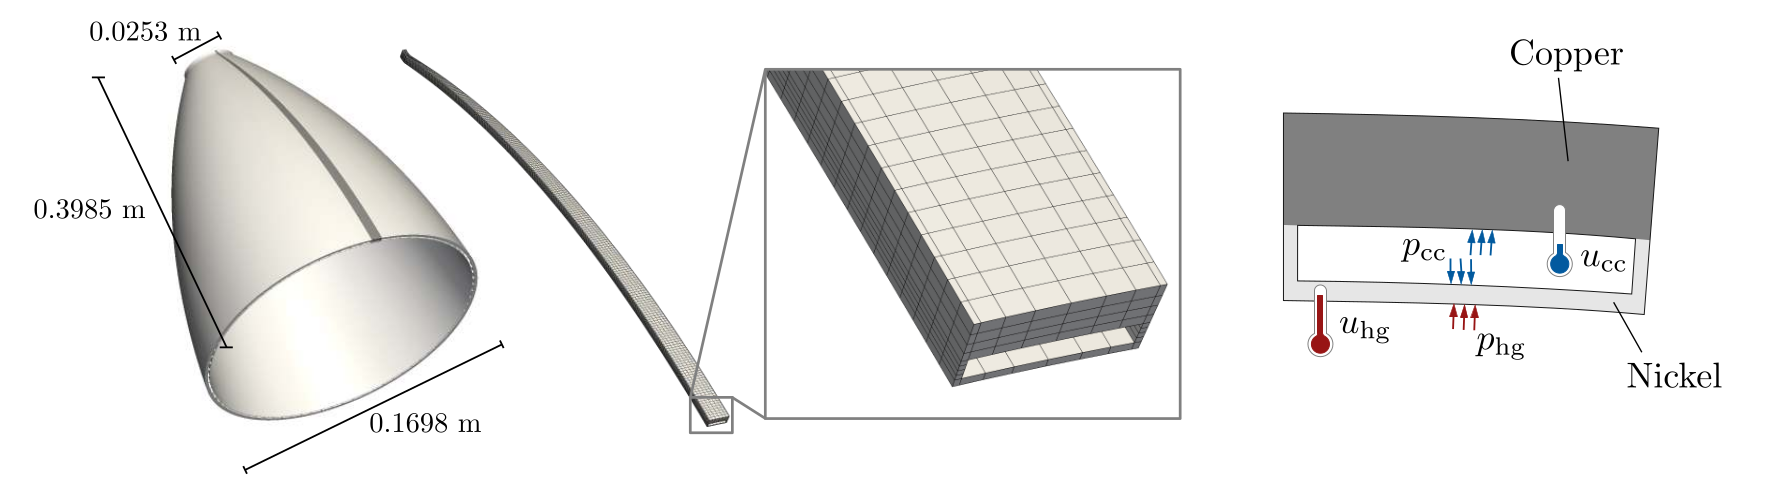
\includegraphics[width=\textwidth]{../_assets/fig12.png}
\caption{Rocket nozzle example: Full geometry of the nozzle (left), computational domain including one cooling channel (center), and generic cross section of the computational domain with the applied thermo-mechanical loads (right). }
\label{fig:tsi-rocket-geom}
\end{figure}

%
\begin{figure}[ht!]
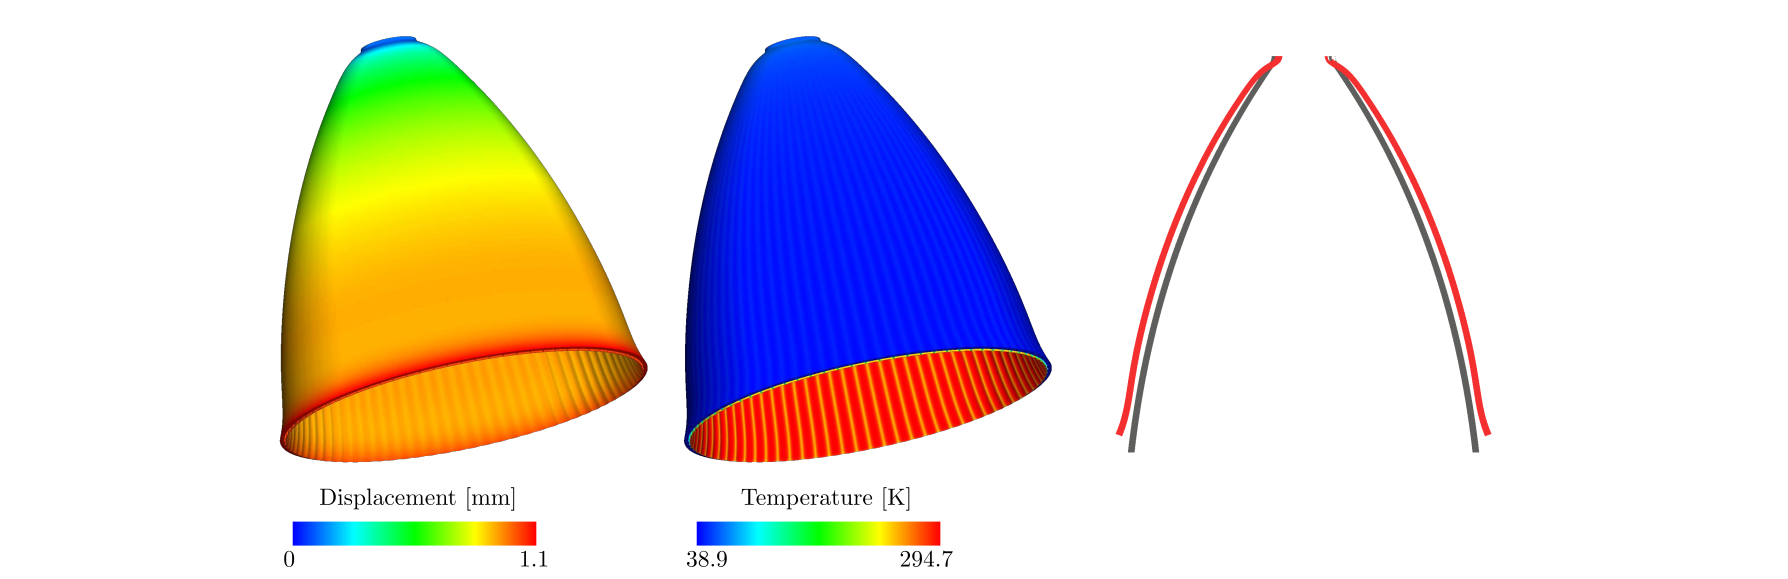
\includegraphics[width=\textwidth]{../_assets/fig13.png}
\caption{Rocket nozzle example: Deformation of the nozzle (left), temperature distribution (center) and original and deformed longitudinal section (right). The results are given at time $t=1$ s and the deformation is magnified 20 times. }
\label{fig:tsi-rocket-sol}
\end{figure}
%
\begin{figure}[ht!]
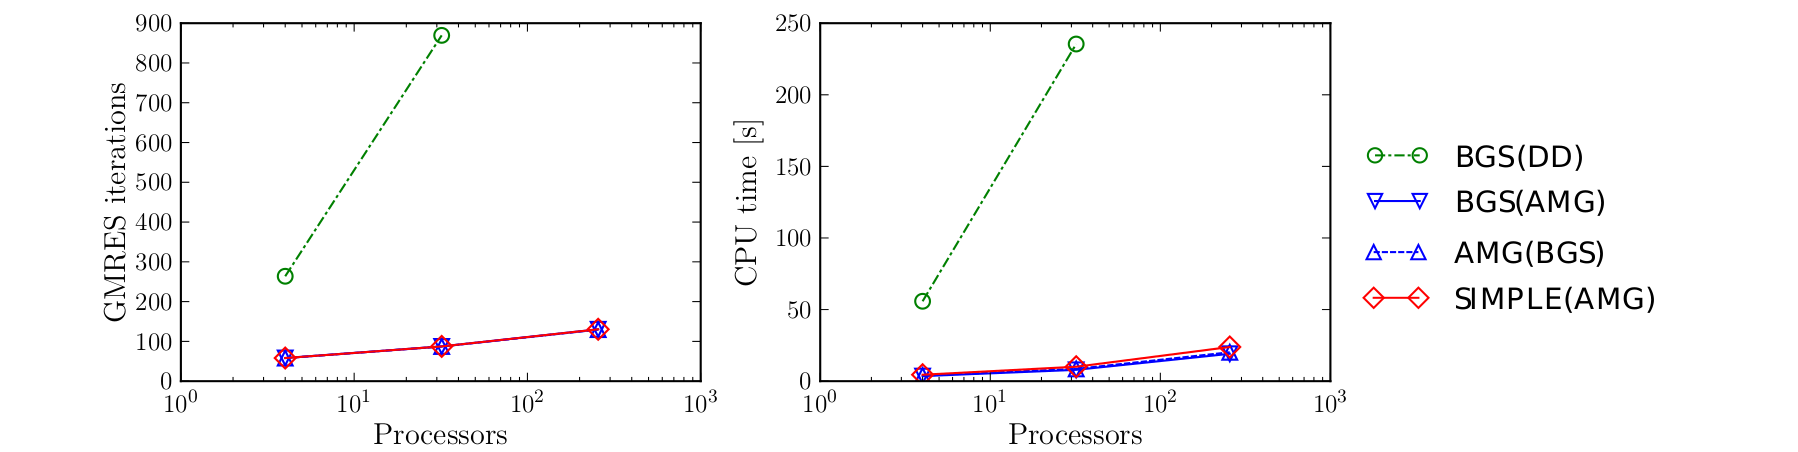
\includegraphics[width=\textwidth]{../_assets/fig14.png}
\caption{Rocket nozzle example: Results of the weak scalability study.  The CPU times include the setup costs of the preconditioner.}
\label{fig:tsi-rocket-weak-scal}
\end{figure}

After the usual space and time discretization, the simulation results into a non-linear problem to be solved at each time step, which is handled with a monolithic Newton scheme. At each Newton iteration, the associated monolithic linear system of equations is solved with a GMRES method preconditioned with four different solvers available in our computational framework. The first method, namely BGS(AMG), considers an outer block Gauss-Seidel (BGS) scheme for uncoupling the fields and then independent \ac{amg} solvers are used to handle the  thermal and mechanical problems separately. The second method, namely SIMPLE(AMG), is a similar method that considers an idea based on the SIMPLE method \cite{Elman2008} for uncoupling the fields instead of BGS. The third method, namely AMG(BGS), is an extension of the monolithic \ac{amg} solver to a generic coupled problem. Finally, the fourth method, namely BGS(DD), is an outer BGS for uncoupling the fields and then standard single-level additive Schwartz preconditioners are used to attack the uncoupled problems. The fourth  method is one of the most simple parallel preconditioners that can be considered in such a problem, and therefore, it is considered here as a reference.  All this solvers could be built easily by means of parameter lists using the general preconditioning framework. 

The performance of the preconditioners is studied with a weak scalability test, see Figure \ref{fig:tsi-rocket-weak-scal}. In this experiment, the ratio between processors and \acp{dof} is kept constant with a value about 12500  DOF/processor. The multi-grid methods AMG(BGS), BGS(AMG) and SIMPLE(AMG) have a very good scalability as the iteration count and CPU time of the linear solver increase only mildly with the problem size. On the other hand, the single-level method BGS(DD) is not scalable since the solver time strongly  grows as the problem size increases. The performance of the single-level method BGS(DD) is particularly poor in this complex example which demonstrates that multi-grid preconditioners such as  AMG(BGS), BGS(AMG) and SIMPLE(AMG) are required in this challenging setting.  In conclusion, the \ac{amg} solvers implemented in our generic computational framework were able to solve this complex example efficiently.

\subsection{Efficient solvers for respiratory mechanics}

Another application of the general linear solver framework has been the simulation of human respiratory mechanics. In recent years, advances have been made towards more protective ventilation strategies \cite{Tobin2001} trying to minimize negative side effects of the treatment, but it is still not fully clear what is the best ventilation strategy for a specific patient. Advanced modeling and simulation offer the possibility of predicting the mechanical response of the respiratory system under different ventilation scenarios, and give an opportunity to design better patient-tailored treatments. However, simulating the human lung poses several computational challenges including large and multiply coupled systems of linear equations. Thus, the underlying motivation of this work is to enable the efficient simulation of virtual lung models on high-performance computing platforms in order to assess mechanical ventilation strategies and contributing to design more protective patient-specific ventilation treatments.

\begin{figure}[ht!]
\centering
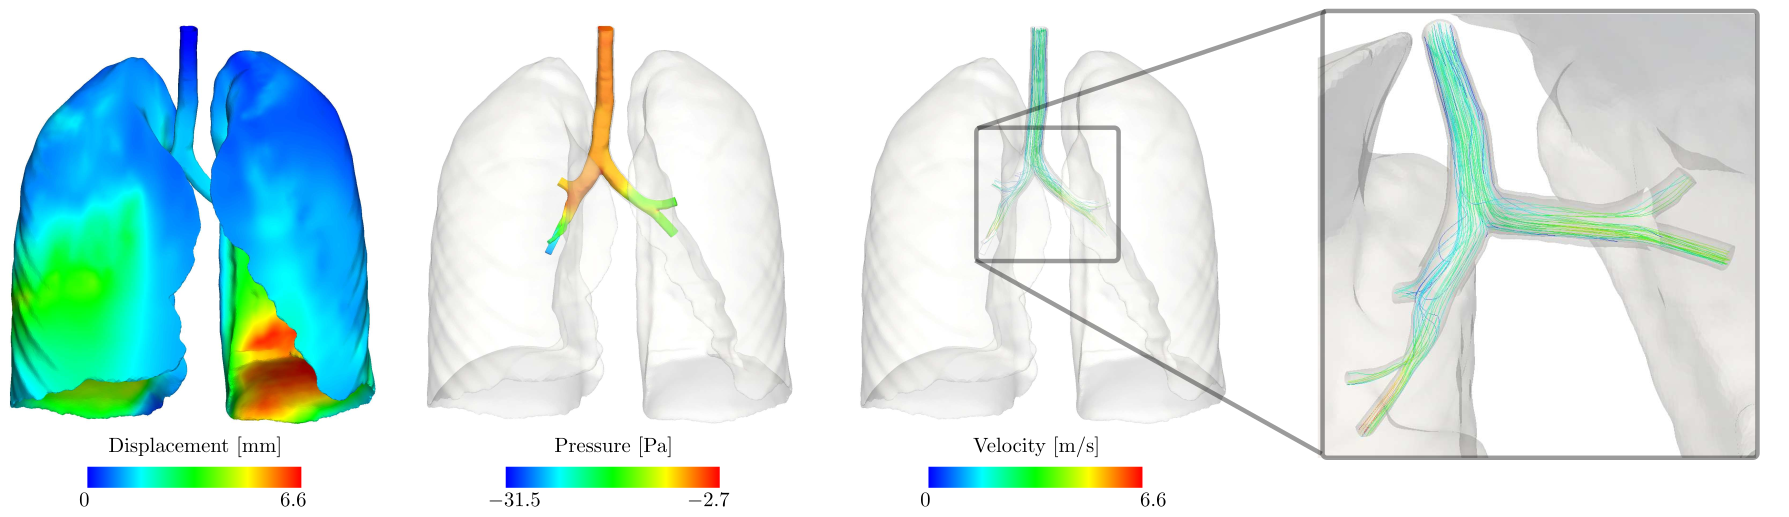
\includegraphics[width=\textwidth]{../_assets/fig15.png}
\caption{Patient-specific lung example: Numerical solution of the lung model consisting of the structural displacement (left), fluid pressure (center) and fluid velocity (right) at time $t=0.75$ s.}
\label{fig:lung-sol}
\end{figure}

The system of linear equations to be solved  in this application is essentially the monolithic system arising in \ac{fsi} extended by additional algebraic constraints. The introduction of these constraints leads to a saddle point problem that cannot be solved with usual \ac{fsi} preconditioners available in the literature. The key ingredient in this work is to use the idea of the semi-implicit method for pressure-linked equations (SIMPLE) for getting rid of the saddle point structure, resulting in a standard \ac{fsi} problem that can be treated with available techniques. Even though the lung model is a complex multi-physics problem (see Figure \ref{fig:lung-sol}), the numerical examples show that the resulting preconditioners approaches the optimal performance (see Figure \ref{fig:medium-lung-scal}). Moreover, the preconditioners are robust enough to deal with physiologically relevant simulations involving complex real-world patient-specific lung geometries. The same approach is applicable to other challenging biomedical applications where coupling between flow and tissue deformation is modeled with additional algebraic constraints. \bemph{This work has lead to 1 paper in a Q1 journal} (see reference \cite{verdugo_efficient_2016}). In the framework of this research, \bemph{I have been junior co-PI in the Bavarian regional project "Efficient solvers for coupled problems in respiratory mechanics"}. 

\begin{figure}[ht!]
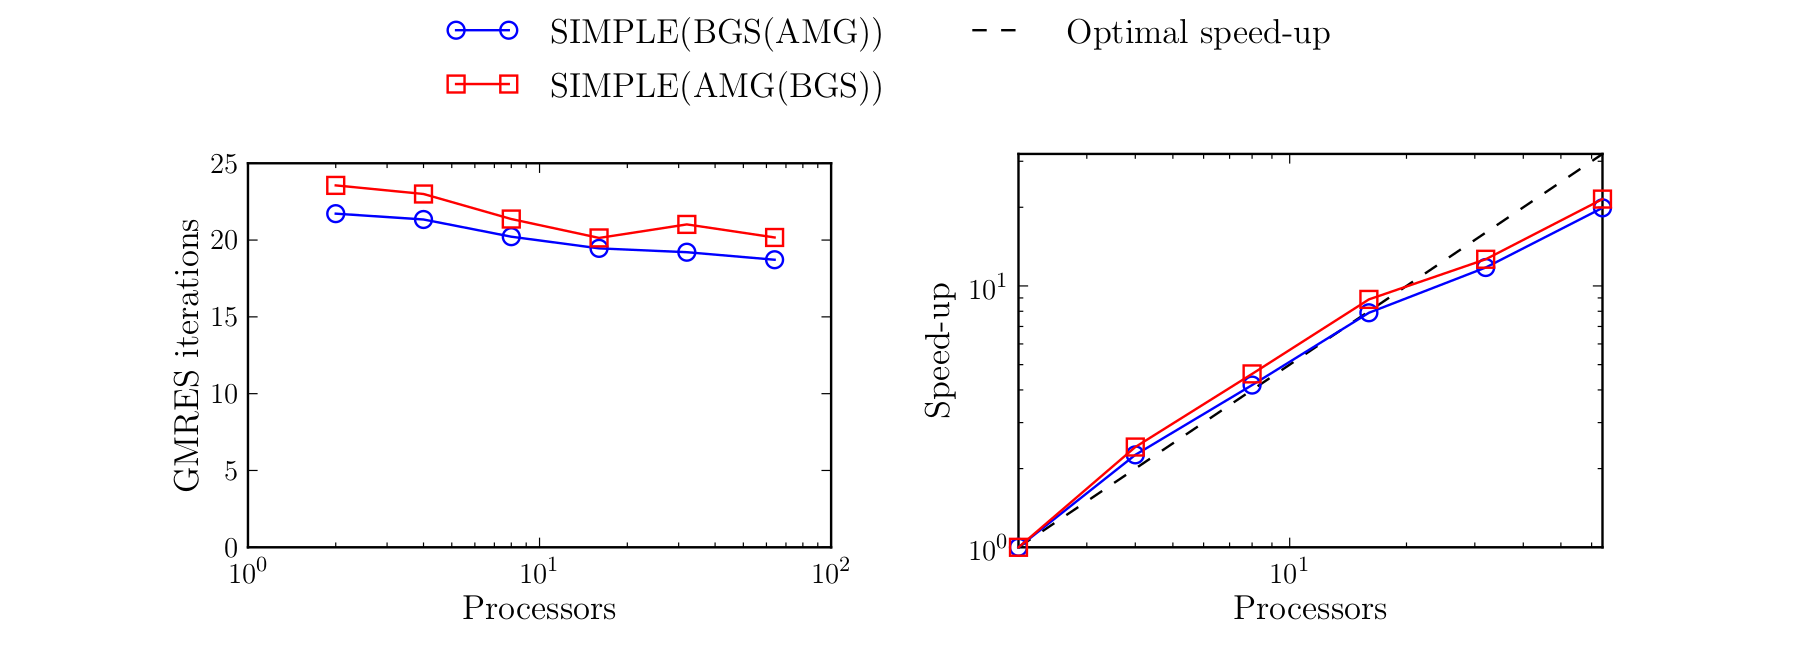
\includegraphics[width=\textwidth]{../_assets/fig16.png}
\caption{Patient-specific lung example: Results of the strong scalability test. The figure shows the dependence of the linear solver iterations with respect to the number of processors (left), and the parallel speed up (right).}
\label{fig:medium-lung-scal}
\end{figure}

 
\section{Pre-doctoral research at UPC (2009-2013)}\label{sec:upc}

\subsection{Thesis overview}

My PhD thesis, entitled ``Error assessment and adaptivity for structural transient dynamics", is devoted to the development of new automatic adaptive mesh refinement tools and goal-oriented error assessment techniques in the context of structural dynamics. Any \ac{fe} based simulation has an intrinsic amount of error with respect to the exact solution of the selected physical model. Being aware of this error is of notorious importance if sensitive engineering decisions are taken on the basis of the numerical results. Assessing the error in elliptic problems (as structural statics) was a well known problem at the time of this PhD thesis. However, assessing the error in other more challenging problem types such as structural transient dynamics was an open research topic. In this context, most of the works provided \emph{a posteriori} error estimates of the energy norm of the discretization error. The challenge was to develop so-called \bemph{goal-oriented} error estimates for this application. That is, \emph{a posteriori} approximations of the error in a given \bemph{quantity of interest} of the underlying physical problem. This goal-oriented error estimation is specially well suited for real-world industrial applications since it provides information of the quality of the computed solution in the targeted quantities instead of a global function norm. 

The main contributions of the PhD thesis are 1) the introduction of a novel technique to compute bounds of the (unknown) discretization error in a given quantity of interest (see reference \cite{verdugo_computable_2012}), 2) a goal-oriented space-time adaptive mesh refinement method specifically designed for efficiency in transient problems (see references \cite{casadei_algorithm_2013,VerdugoParesDiez2014a}), and 3)  a novel paradigm for error estimation in transient problems based on a new type of quantities of interest (see reference \cite{Verdugo2013}). I published a review paper with my main thesis results (see reference \cite{verdugo_error_2014}) in the "Archives of Computational Methods in Engineering", which is the \bemph{1st ranked journal} in the category "mathematics, interdisciplinary applications" of the Journal Citation Reports (JCR) in the year of publication. In the following, I briefly introduce items 2) and 3), which are the major thesis novelties.

\subsection{Modal-based goal-oriented error assessment and adaptive mesh refinement}

Goal-oriented error estimation and adaptivity is particularly challenging in time-dependent problems. Assessing the error in the quantity of interest requires introducing an auxiliary problem, referred to as the adjoint or dual problem \cite{becker_optimal_2001}. The main difficulty is associated with the fact that the adjoint solution has to be solved backwards in time. This means that, in order to assess the error by weighting the residual of the direct (or forward) solution with the adjoint (or backward) solution, at least one of the two solutions have to be stored in the full time-space domain. In non-linear problems, the situation is even worse because the full forward problem has to be computed and stored to define the backwards adjoint. This means that assessing the error of each iteration of the forward problem potentially requires computing a different backward adjoint. The conventional approach to alleviate the storage requirements is to use \emph{checkpointing} (see \cite{Griewank2000}), where the forward solution is stored only at a small number of pre-selected time points. These stored snapshots are used  as initial conditions on each sub-interval for recomputing the forward solution during the backwards adjoint computation. This approach mitigates the storage requirements, but for some applications, recomputing the forward solution repeatedly can be still too expensive.

\begin{figure}[ht!]
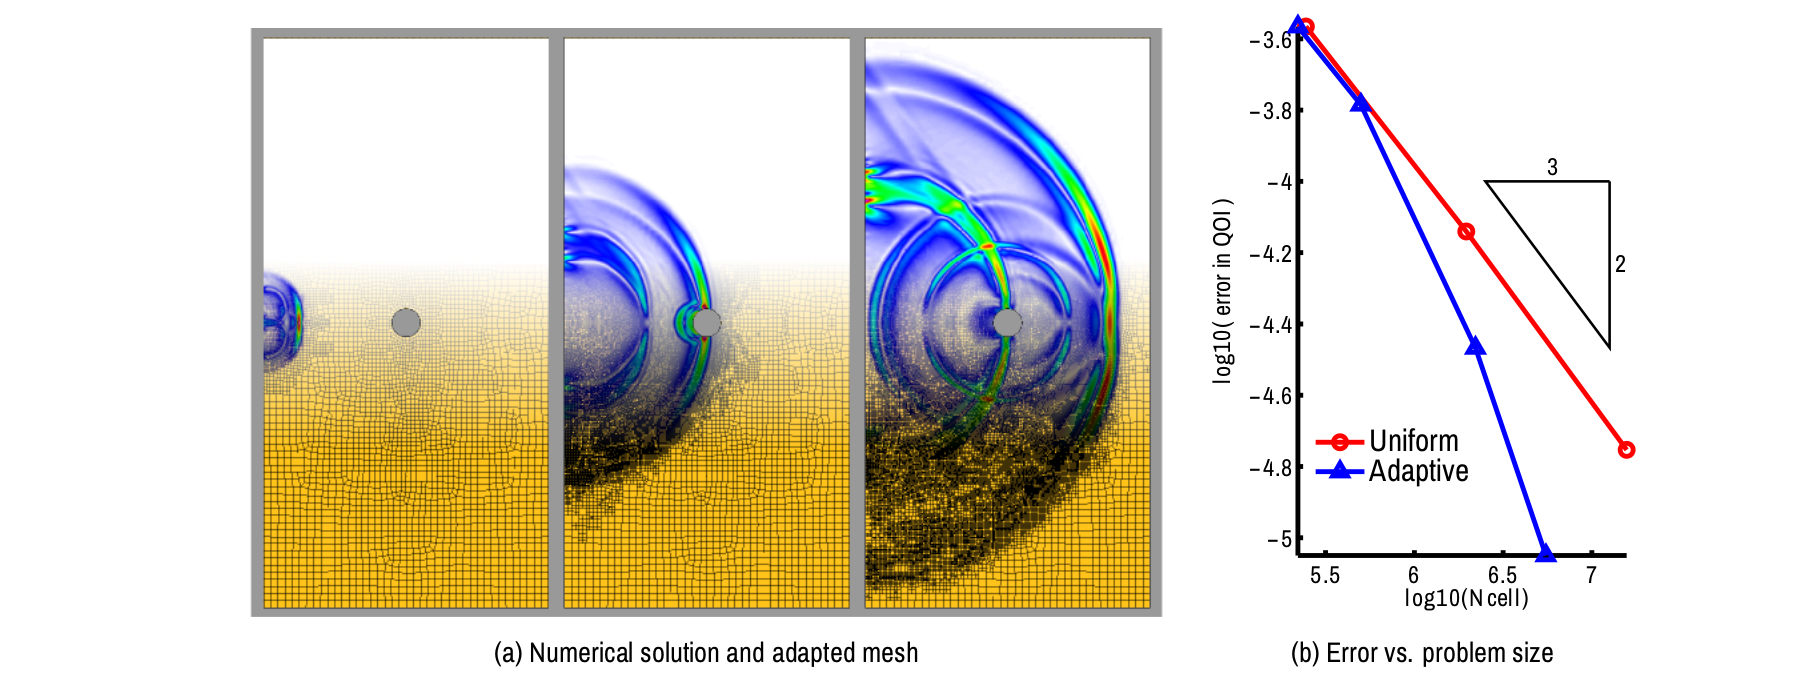
\includegraphics[width=\textwidth]{../_assets/fig17.png}
\caption{Simulation of elastic waves propagating in a perforated plate. The underlying space-time discretization has been automatically adapted using the goal-oriented error estimators in \cite{Verdugo2013}. A smaller number of mesh elements are required with the adapted meshes than with uniform discretizations in order to achieve the same level of accuracy. }
\label{fig:amr-phd}
\end{figure}

In the thesis, I have proposed an alternative approach based on a well known technique for structural dynamics: modal analysis. The modal-based strategy is particularly well suited for computing the adjoint problem associated with some particular quantities of interest. Following this approach, the adjoint solution is computed and stored for each vibration mode instead of for each time step, which reduces the storage requirements enormously. Using this novel approach, one can compute efficiently local error indicators that for each element and time step in the chosen discretization. This information can be used to automatically increase the resolution of the space and time discretizations only in the regions, where it is actually needed, leading to efficient computations (see Figure \ref{fig:amr-phd}). 


\subsection{A novel a-posteriori error estimation paradigm based on time-line dependent quantities of interest}

Virtually all the literature on goal-oriented \emph{a posteriori} error assessment is based on scalar quantities of interest. While this approach is well suited for steady-state problems, a single scalar value does not give enough pieces of information about a complex space-time solution. For this reason, the preferred quantities of interest in time-dependent problems are typically the history (or evolution) of the space average of the solution in a sub-region of the domain, which are referred to as time-line dependent quantities of interest \cite{Verdugo2013}. At the time of this PhD thesis, there was no error estimation method for this kind of quantities in the literature. One of the main thesis contributions is a new paradigm for \emph{a posteriori} error estimation using this new type of quantities of interest.

As already announced, in conventional goal-oriented error assessment in a given scalar quality, one needs to introduce and solve an adjoint problem. Dealing with time-line dependent quantities is much more challenging. A time-line dependent quantity can be understood as a family of infinite scalar quantities (one for each time point in the selected computation time interval).  Thus, one needs the solution of a family of infinite adjoint problems. This is computationally un-affordable in practice. However, for a number of meaningful cases, I have mathematically proven in reference \cite{Verdugo2013} that all this adjoint problems are the equivalent after a translation of the time variable. This fundamental result is the crucial observation that allows one to assess the error in the time-line dependent quantities with an affordable cost. In addition, using a modal-based approximation of the adjoint problem allows one to accurately estimate the error in this new type of quantities in an efficient way (see Figure \ref{fig:tl-qoi} ).


\begin{figure}[ht!]
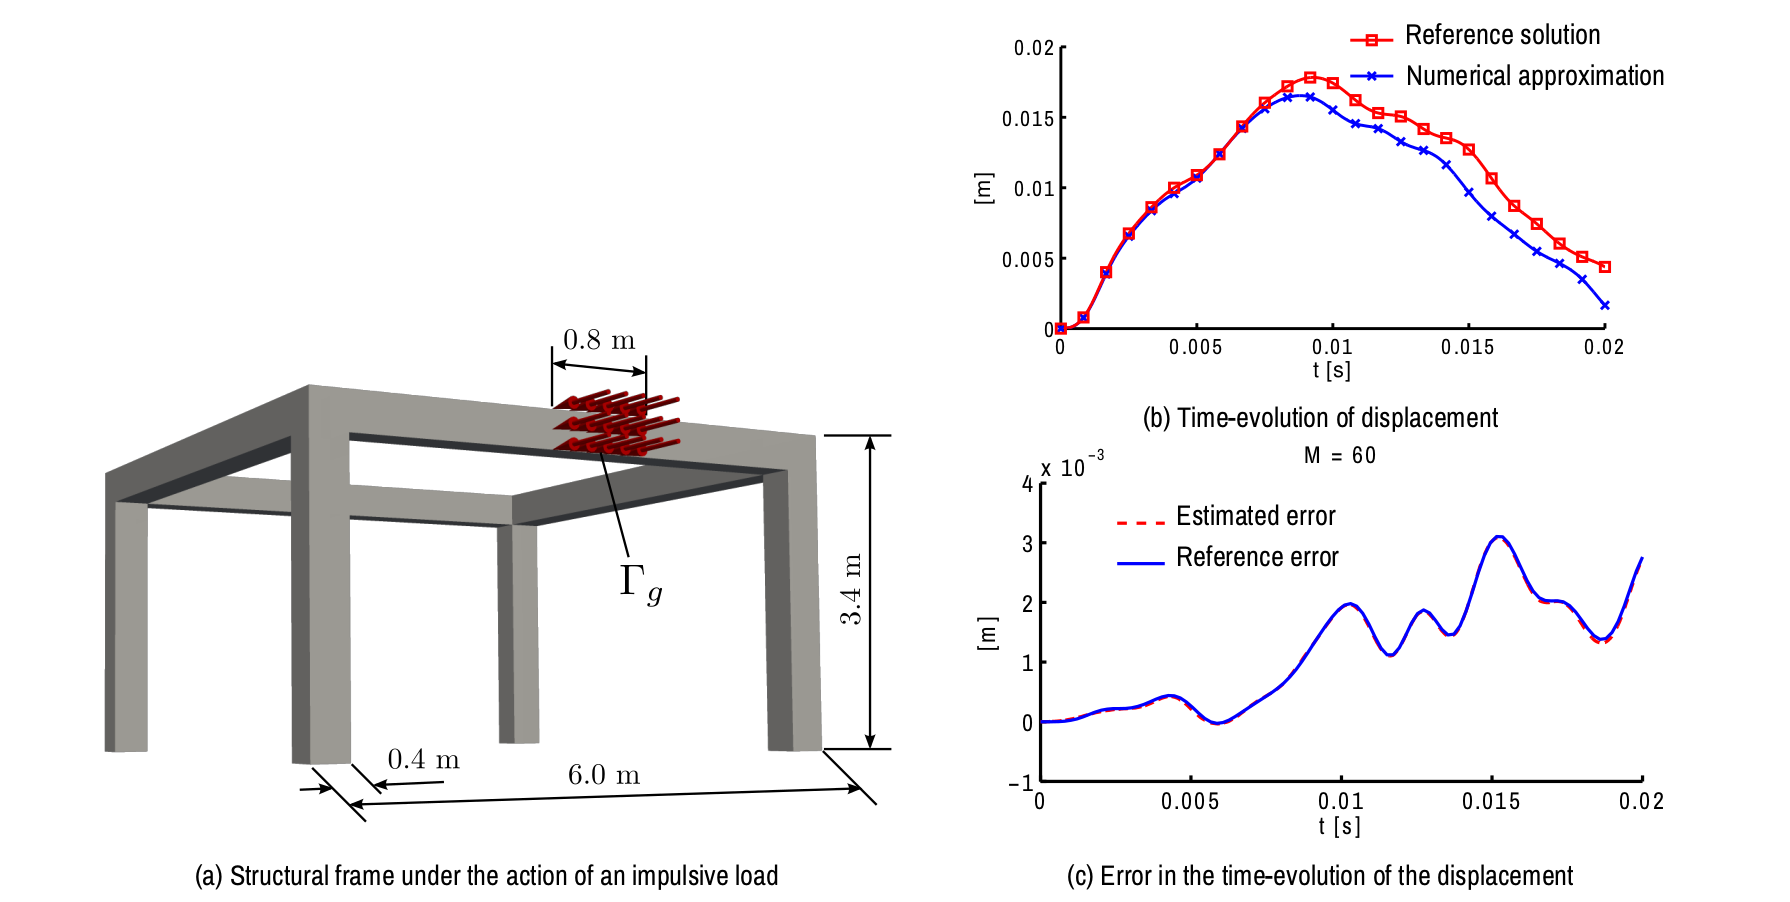
\includegraphics[width=\textwidth]{../_assets/fig18.png}
\caption{Error estimation of a time-line dependent quantity of interest (in this case the time-evolution of the averaged displacement at region $\Gamma_g$). Note that by approximating the family of adjoint problems associated with this quantity using only 60 vibration modes, an accurate estimation of the numerical error is achieved. }
\label{fig:tl-qoi}
\end{figure}

 
 
 

%\setlength{\bibsep}{0.0ex plus 0.00ex}
\bibliographystyle{myabbrvnat}
\bibliography{refs.bib}

\end{document}